\documentclass[a4paper]{article} %format de la feuille + type de document https://en.wikibooks.org/wiki/LaTeX/Document_Structure#Document_classes
%packages nécessaire pour nos besoins
\usepackage[utf8]{inputenc}
\usepackage[T1]{fontenc}
\usepackage[english,french]{babel}
\usepackage{amsmath}
\usepackage{amssymb,amsfonts,textcomp}
\usepackage{color}
\usepackage{array}
\usepackage{hhline}
\usepackage{hyperref}
\usepackage[pdftex]{graphicx}
\usepackage{sectsty}
\usepackage{tcolorbox}
\usepackage{textcomp}
\usepackage{courier}
\usepackage[font={small,it}]{caption}
\usepackage{float}
\usepackage{graphicx}
\usepackage{caption}
\usepackage{tabularx}
\usepackage{multirow}% http://ctan.org/pkg/multirow
\usepackage{tikz}
\usepackage[top=15mm,bottom=20mm,right=50mm,left=50mm]{geometry} 
\usepackage[export]{adjustbox}


%Définition des couleurs
\definecolor{havelockBlue}{rgb}{0.004, 0.42, 0.73}
\definecolor{Monokaimagenta}{rgb}{0.86,0.08,0.24}

%utilisation de la couleur définie avant
%toutes les sections auront cette couleur
\sectionfont{\color{havelockBlue}}
%\subsectionfont{\color{havelockBlue}}
%début du document
\begin{document}

\renewcommand{\labelitemi}{$\bullet$}
\renewcommand{\labelitemii}{$\cdot$}
\renewcommand{\labelitemiii}{$\diamond$}
\renewcommand{\labelitemiv}{$\ast$}

%début d'un titre
\begin{titlepage}
            %centre les éléments
	\centering
	
	{\scshape\LARGE \color{Monokaimagenta} Laboratoire \\  \par}
	
	%espace vertical de 1 mms
	\vspace{1cm}
	
	{\Large\itshape Sven Rouvinez \& Johanna Melly\par}
	
	%http://www.personal.ceu.hu/tex/spacebox.htm
	\vfill
	Professeur\par
	%met le texte en gras 
	\textbf{Carlos Andrés Pena} \par% ajoute une ligne 
	\vspace{1cm}
	Assistant\par
	\textbf{Gaëtan Matthey}
	
	\vfill

            %affiche la date actuelle
	{\large \today\par}
	
%fin de la page de titre
\end{titlepage}

\section{Objectifs du laboratoire}
Ce laboratoire consistait en la réalisation d'un décodeur, qui comprenait aussi une partie gérant les instruction MOV et ADD. Son bon fonctionnement devait être testé à l'aide du main fourni dans le workspace du laboratoire.

\section{Blocs Logisim étapes 1 à 3}
Il y avait 2 circuits logisim à rendre pour ce labo, cette partie traite des étapes concernant la mise en place du système et uniquement du traitetement de l'instruction MOV, à la partie 2 s'ajoute l'instruction ADD.\\
Nous avons donc décidé de séparer les blocs afin de permettre une meilleure modularité et abstraction du système DECODE.\\
\paragraph{Résumé}
\begin{itemize}
    \item     MOV\_INST détecte une instruction \textbf{MOV}
    \item     REGISTER\_16BITS contient les registres (banque de registres)
    \item     DECODE décode les instructions \textbf{MOV} et \textbf{ADD} et les transmet à la banque de registre
    \item     main le bloc principal, avec la mémoire contenant les instructions, et le \textbf{DECODE}
\end{itemize}

\subsection{MOV\_INST}
Cette instruction MOV Rd, Rn est en fait une instruction ADD\ref{addinst} Rd, Rn, \#0 mais le champ de la valeur immédiate de celui-ci est mis à 0.
\begin{figure}[H]
    \centering
    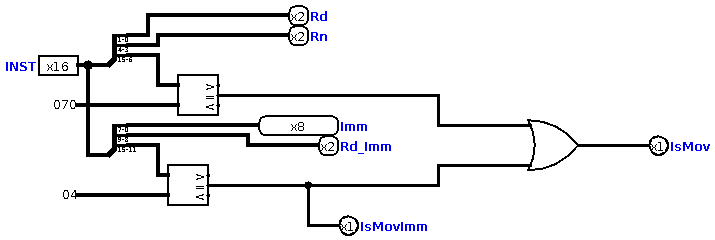
\includegraphics[width=.8\textwidth]{src/MOV_INST.png}
    \caption{Instruction MOV}
    \label{mov_img}
\end{figure}
\paragraph{Définition des entrées:}
\begin{itemize}
    \item     INST: code complet
    \item     0x70: code recherché pour un MOV avec un registre comme destination
    \item     0x04: code recherché pour un MOV avec valeur immédiate
\end{itemize}

\paragraph{Définition des sorties:}
\begin{itemize}
    \item     Rd: registre destination
    \item     Rn: registre source
    \item     IsMov: s'active si les bits de 15 à 9 sont égaux à $0001110000$ (0x070) ou à $0000010$ (0x04).
    \item     Imm: valeur immédiate
    \item     Rd\_Imm: registre destination pour MOV avec valeur immédiate
    \item     IsMovImm: s'active s'il y a un MOV avec valeur immédiate

\end{itemize}

\medskip

Ce bloc permet de détecter si une instruction \textbf{MOV} est trouvée, grâce au comparateur dans le code de sortie de la ROM.
\\Cette instruction va charger la valeur du registre source (Rn) dans le registre destination (Rd).\\
Elle se caractérise par le code ci-dessous : 
\\
\begin{tabular}{|ccccccc|ccc|ccc|ccc|}
    \hline
    \multicolumn{7}{|c|}{Code ARM}  & \multicolumn{3}{|c|}{Opcode} & \multicolumn{3}{|c|}{Rn} & \multicolumn{3}{|c|}{Rd}\\
    \hline
    15 & 14 & 13 & 12 & 11 & 10 & 9 & 8 & 7 & 6                    & 5 & 4 & 3                & 2 & 1 & 0 \\
    \hline
    0  & 0  & 0  & 1  & 1  & 1  & 0 & 0 & 0 & 0                    & \multicolumn{3}{|c|}{}   &\multicolumn{3}{|c|}{}\\
    \hline     
    \end{tabular}
\\

\begin{itemize}
    \item     Code ARM : instruction ARM à effectuer
    \item     Opcode : instruction à effectuer par l'ALU
    \item     Rn : registre source
    \item     Rd : registre destination
\end{itemize}

\medskip
Nous avons donc deux codes ARM différents, selon la valeur donnée pour Rd, qui peut être une valeur immédiate ou non. Ainsi, dans ce bloc, la sortie \textbf{IsMovImm} va indiquer le si l'instruction indique un registre ou une valeur. 
\\La sortie \textbf{IsMov} va être activée, indépendamment de s'il s'agit d'une valeur immédiate ou non, puisqu'elle indique uniquement s'il y a eu une instruction MOV.



    
\subsection{REGISTER\_16BITS} \label{regi16}
Ce bloc permet de stocker et retourner les différentes valeurs des instructions transmises.

\begin{figure}[H]
    \centering
    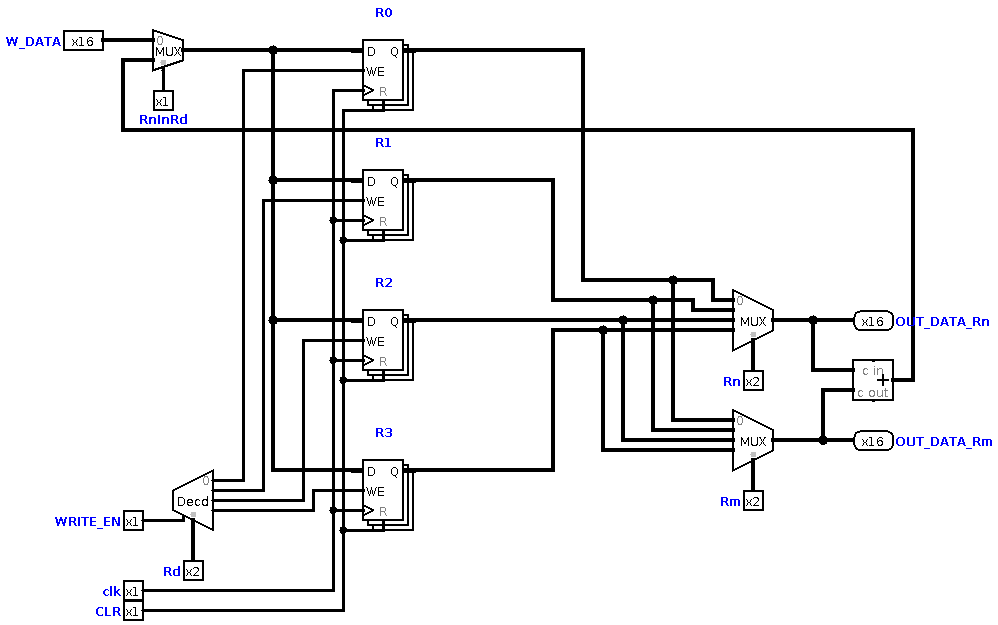
\includegraphics[width=.8\textwidth]{src/REGISTERS_16BITS.png}
    \caption{Banque de registres}
    \label{regi16_img}
\end{figure}



\paragraph{Définition des entrées:}
\begin{itemize}
    \item     W\_DATA: contient les données à entrer
    \item     WRITE\_EN: active l'écriture
    \item     clk: horloge
    \item     CLR: reset
    \item     Rd: registre destination
    \item     Rn: registre source
    \item     RnInRd: est actif si pas de valeur immédiate
\end{itemize}
\paragraph{Définition des sorties:}
\begin{itemize}
    \item OUT\_DATA\_Rn: valeur du registre choisi
\end{itemize}

\medskip
Il permet de choisir s'il faut travailler avec une valeur d'un registre ou une valeur immédiate, une choisissant le registre (Rd) dans lequel inscrire les données, et une permettant la sortie des adresses (Rn), selon le registre.
Ainsi, les données sont reçues en entrée \textbf{W\_DATA} qui selon l'instruction vont être issue d'une valeur existante dans un registre ou une donnée immédiate via l'offset. 
\\Si l'entrée \textbf{WRITE\_EN} est active, alors l'élément decode va permettre l'écriture dans un registre choisi (grâce à \textbf{Rd}) des données.


\subsection{DECODE}
Ce bloc est l'élément principal de notre circuit, il aiguille les instructions et leur données dans les registres corrects.
Afin de permettre une abstraction complète des systèmes entre eux, nous avons décidé d'utiliser des extenders de $n \rightarrow 16$ bits.\\
\begin{figure}[H]
    \centering
    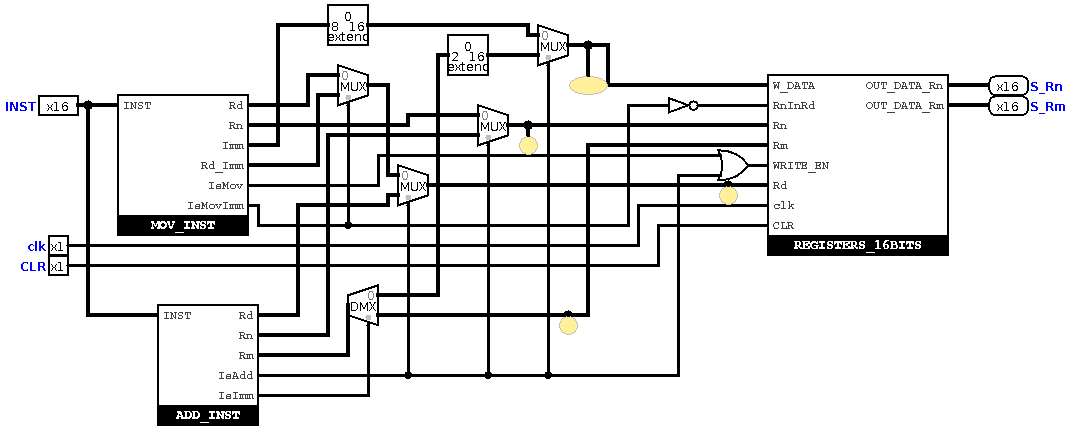
\includegraphics[width=1\textwidth]{src/DECODE.png}
    \caption{Decode}
    \label{decode_img}
\end{figure}

\paragraph{Définition des entrées:}
\begin{itemize}
    \item     INST: instruction à effectuer
    \item     clk: horloge
    \item     CLR: reset
\end{itemize}

\paragraph{Définition de la sortie:}
\begin{itemize}
    \item     S\_Rn: Registre source
\end{itemize}
\medskip
Les sorties des blocs \textbf{MOV\_INST} étant toutes reliées à des entrées du bloc \textbf{REGISTERS\_16BITS}, le circuit \textbf{DECODE} sera expliqué en décrivant les liens entre les 2 circuits.\\

\paragraph{W\_DATA:} 
Cette entrée est reliée à la sortie Imm du \textbf{MOV\_INST}. Elle va prendre la valeur immédiate en sortie de MOV, selon l'instruction donnée. Cette sortie correpond à la valeur immédiate de l'instruction MOV et est sur 8 bit, elle passe donc dans un extendeur qui permet de passer à 16 bits. S

\paragraph{RnInRd:} 
Prend en entrée une négation du IsMovImm, qui indique que la valeur de l'instruction MOV n'est pas immédiate et donc la valeur à récupérer se trouve dans un registre.

\paragraph{Rn:}
Le Rn du \textbf{MOV\_INST} est connecté en direct au Rn du \textbf{REGISTER\_16BITS}

\paragraph{WRITE\_EN:}
Activée s'il y a une instruction MOV détectée

\paragraph{Rd:}
L'entrée Rd du \textbf{REGISTER\_16bits} prend en entrée la sortie Rd du bloc \textbf{MOV\_INST} ou si valeur immédiate il y a, Rd\_Imm, selon les données de l'instruction\\

Les deux dernières entrées du bloc (clk et CLR) sont simplement l'horloge et le reset.




\subsection{main}
\begin{figure}[H]
    \centering
    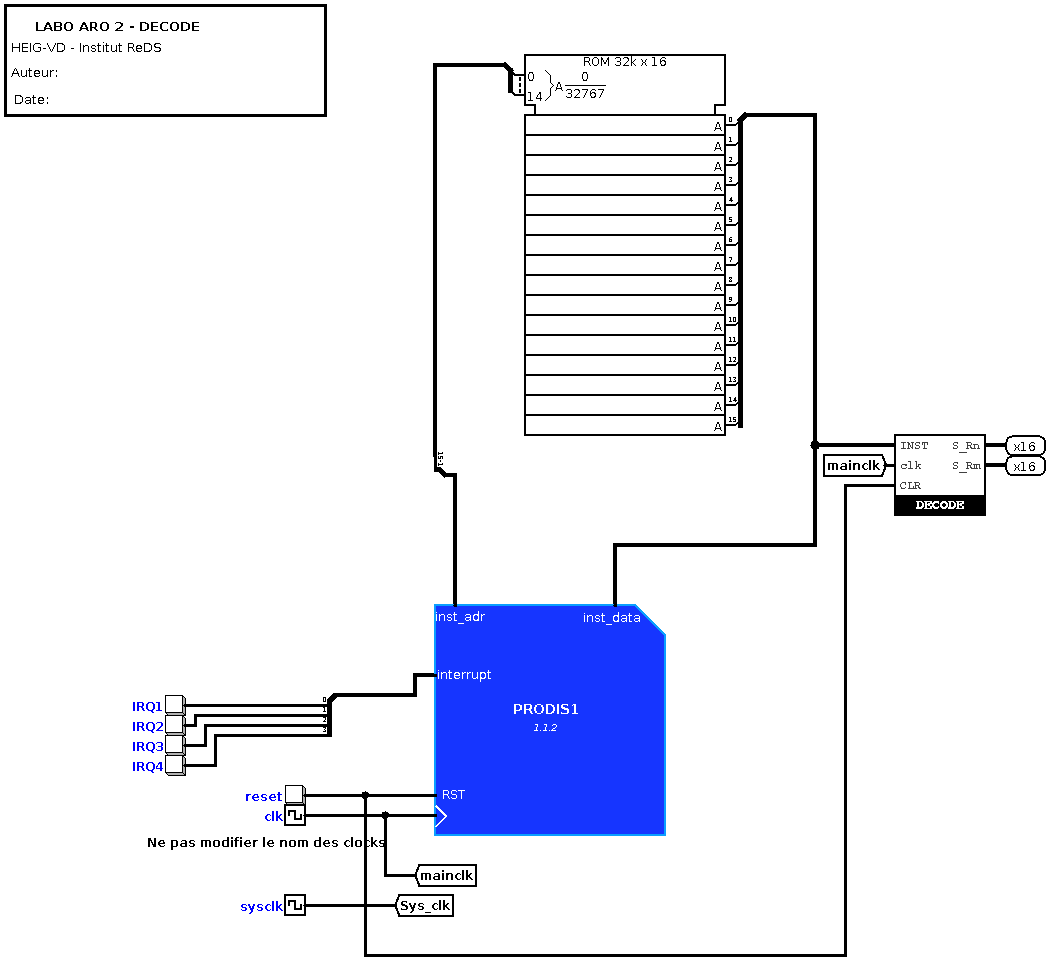
\includegraphics[width=1\textwidth]{src/main.png}
    \caption{Main program}
    \label{main_img}
\end{figure}

Le circuit main nous a permis de contrôler le bon fonctionnement de notre \textbf{DECODE}. Notre fichier main.S contenait comme instructions:\\

\begin{tabular}{|c|c|c|c|}    
    \hline
    INST & Rd & Rn \\
    \hline
    MOV  & r0 & \#27    \\
    \hline
    MOV  & r2 & \#4    \\
    \hline
    MOV  & r3 & \#67    \\
    \hline
    MOV  & r1 & r3  \\
    \hline
    MOV  & r0 & r2 \\
    \hline
    MOV  & r1 & 0xAC    \\
    \hline
\end{tabular}

\pagebreak
Le chronogramme suivant a permis de contrôler la bonne éxécution des instructions présentes dans le fichier fourni main.S décrit ci-dessus.\\
Toutes les valeurs sont en hexadécimal.
\begin{itemize}
    \item     INST: instruction courante
    \item     R0 à R3: registre et leur valeur
    \item    W\_DATA: valeur immédiate courante si utilisé
    \item    OUT\_DATA: sortie actuelle de la banque de registre
    \item    Rd: Registre destination utilisé
    \item    Rn: Registre source utilisé
\end{itemize}

\begin{figure}[h]
    \centering
    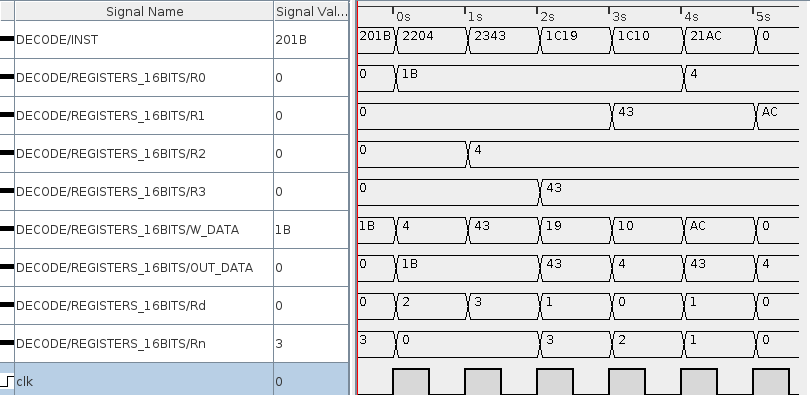
\includegraphics[width=1.3\textwidth]{src/CHRONO_MAIN.png}
    \caption{Chonogramme decode}
    \label{chrono_decode}
\end{figure}
\pagebreak

\paragraph{Afin de tester} les valeurs de notre circuit, un autre tableau avec les valeurs des registres qui changent pendant le fonctionnement:\\

\begin{tabular}{|c|c|c|c|c|}    
    \hline
    Temps (coup de clk) & $R_0$ & $R_1$          & $R_2$          & $R_3$ \\
    \hline
    0                   & 0     & 0              & 0              & 0 \\
    \hline
    1                   & \textbf{27}            & 0     & 0     & 0   \\
    \hline
    2                   & 27    & 0              & \textbf{4}     & 0 \\
    \hline
    3                   & 27    & 0              & 4              & \textbf{67}  \\
    \hline
    4                   & 27    & \textbf{67}    & 4     & 67\\
    \hline
    5                   & \textbf{27}    & 67    & 27    & 67 \\
    \hline
    6                   & 27    & \textbf{172}    & 27    & 67\\
    \hline
\end{tabular}

    
    
\section{Blocs Logisim étape 4}
Les blocs existants du chapitre ci-dessus sont repris mais ne seront pas décrit ici, sauf si des changements ont dû être fait.
\paragraph{Résumé}
\begin{itemize}
    \item     MOV\_INST détecte une instruction \textbf{MOV}
    \item     ADD\_INST détecte une instruction \textbf{ADD}
    \item     REGISTER\_16BITS banque de registres
    \item     DECODE Décode les instructions \textbf{MOV} et \textbf{ADD} et les transmet à la banque de registre
    \item     main le bloc principal, avec la mémoire contenant les instructions, et le \textbf{DECODE}
\end{itemize}

\subsection{MOV\_INST}

\begin{figure}[H]
    \centering
    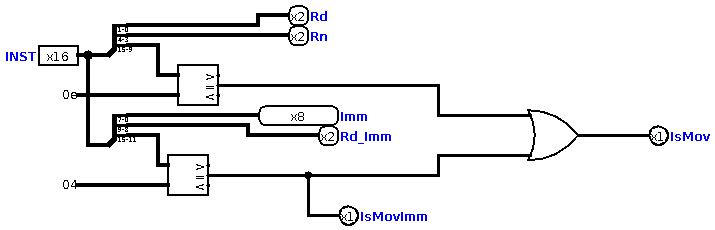
\includegraphics[width=.8\textwidth]{src/Et4_MOV_INST.png}
    \caption{Instruction MOV}
    \label{mov_img}
\end{figure}
\paragraph{Définition des entrées:}
\begin{itemize}
    \item     INST: code complet
    \item     0x0e: code recherché pour un MOV avec valeur non immédiate
    \item     0x04: code recherché pour un MOV avec valeur immédiate
\end{itemize}

\paragraph{Définition des sorties:}
\begin{itemize}
    \item     Rd: registre destination
    \item     Rn: registre source
    \item     IsMov: s'active si les bits de 15 à 9 sont égaux à $0001110$ (0x0e) ou à $0000010$ (0x04).
    \item     Imm: valeur immédiate
    \item     Rd\_Imm: registre destination pour MOV avec valeur immédiate
    \item     IsMovimm: s'active si on a un MOV avec valeur immédiate

\end{itemize}

\medskip

Ce bloc permet de détecter si une instruction \textbf{MOV} est trouvée, grâce au comparateur, dans le code de sortie de la ROM, cette instruction va charger la valeur du registre source (Rn) dans le registre destination (Rd).\\
Elle se caractérise par le code ci-dessous : 
\\
\begin{tabular}{|ccccccc|ccc|ccc|ccc|}
    \hline
    \multicolumn{7}{|c|}{Code ARM}  & \multicolumn{3}{|c|}{Opcode} & \multicolumn{3}{|c|}{Rn} & \multicolumn{3}{|c|}{Rd}\\
    \hline
    15 & 14 & 13 & 12 & 11 & 10 & 9 & 8 & 7 & 6                    & 5 & 4 & 3                & 2 & 1 & 0 \\
    \hline
    0  & 0  & 0  & 1  & 1  & 1  & 0 & 0 & 0 & 0                    & \multicolumn{3}{|c|}{}   & \multicolumn{3}{|c|}{}\\
    \hline     
    \end{tabular}
\\

\begin{itemize}
    \item     Code ARM : instruction ARM à effectuer
    \item     Opcode : instruction à effectuer par l'ALU
    \item     Rn : registre source
    \item     Rd : registre destination
\end{itemize}

\medskip
Nous avons donc deux codes ARM différents, selon la valeur donnée pour RD, qui peut être une valeur immédiate (en héxadécimal). Ainsi, dans ce bloc, on a les sorties correspondant au registres et valeurs concernées, et on peut vérifier le type de donnée grâce à la sortie \textbf{IsMovImm} qui va indiquer le type de donnée. La sortie \textbf{IsMov} va être activée, indépendamment de s'il s'agit d'une valeur immédiate ou non, puisqu'elle indique uniquement s'il y a eu une instruction MOV.



\subsection{ADD\_INST} \label{addinst}
\begin{figure}[H]
    \centering
    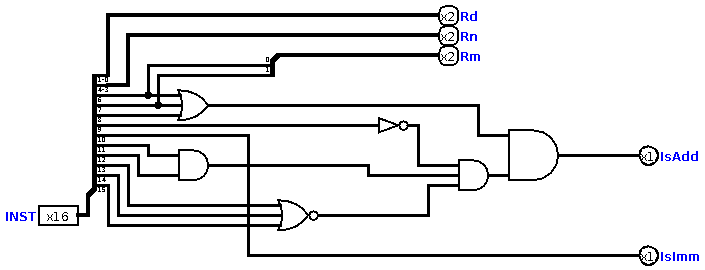
\includegraphics[width=.8\textwidth]{src/Et4_ADD_INST.png}
    \caption{Instruction ADD}
    \label{add_img}
\end{figure}

\paragraph{Définition des entrées:}
\begin{itemize}
    \item     INST: code complet
\end{itemize}

\paragraph{Définition des sorties:}
\begin{itemize}
    \item     Rd: registre destination
    \item     Rn: registre source 2
    \item     Rm: registre source 1
    \item     IsAdd: s'active si l'instruction ADD est détectée
    \item     IsImm: s'active s'il y a une valeur immédiate
\end{itemize}
\medskip 

L'instruction ADD est présente sous 2 formes:
\paragraph{ADD Rd, Rn, \#$imme_3$}\mbox{}\\
\begin{tabular}{|ccccccc|ccc|ccc|ccc|}
    \hline
    \multicolumn{7}{|c|}{Code ARM}  & \multicolumn{3}{|c|}{$imme_3$} & \multicolumn{3}{|c|}{Rn} & \multicolumn{3}{|c|}{Rd}\\
    \hline
    15 & 14 & 13 & 12 & 11 & 10 & 9 & 8   & 7   & 6                  & 5 & 4 & 3                & 2   & 1   & 0 \\
    \hline
    0  & 0  & 0  & 1  & 1  & 1 & 0  &  \multicolumn{3}{|c|}{}        &  \multicolumn{3}{|c|}{}  & \multicolumn{3}{|c|}{} \\
    \hline     
    \end{tabular}

\paragraph{ADD Rd, Rn, Rm}\mbox{}\\
\begin{tabular}{|ccccccc|ccc|ccc|ccc|}
    \hline
    \multicolumn{7}{|c|}{Code ARM}  & \multicolumn{3}{|c|}{Rm} & \multicolumn{3}{|c|}{Rn} & \multicolumn{3}{|c|}{Rd}\\
    \hline
    15 & 14 & 13 & 12 & 11 & 10  & 9 & 8   & 7   & 6                 & 5 & 4 & 3                & 2   & 1   & 0 \\
    \hline
    0  & 0  & 0  & 1  & 1  & 0   & 0 &  \multicolumn{3}{|c|}{}     &  \multicolumn{3}{|c|}{}  & \multicolumn{3}{|c|}{} \\
    \hline     
    \end{tabular}    

\vspace{1cm}    
    Le circuit ADD fonctionne ce cette manière: les bits 15-13 doivent être à 0, et passent donc dans une porte NOR. Si la sortie est à 1, c'est que les 3 bits sont à zéro (ce que l'on cherche ici). Les bits 12-11, quant à eux, doivent être à 1. Ils passent donc dans une porte AND pour vérifier que ce soit le cas. Le bit 10 indique s'il d'agit d'une valeur immédiate (1) ou non (0). Le bit 9 insique s'il agit d'un ADD (0) ou d'un SUB (1), ainsi, il est suivi d'un NOT pour obtenir un 1 s'il s'agit bien d'une instruction ADD. Les bits 8-6 correspondent à l'offset, et les bits 7-6 au registre source 1 s'il n'y a pas de valeur immédiate. Les bits 4-3 correspondent au registre source 2, et les bits 1-0 au registre destination.
    La sortie est précédé d'un porte AND qui vérifie que les critères permettant de reconnaître qu'il s'agit bien de l'instruction recherchée.
    
    
\subsection{DECODE}
\begin{figure}[H]
    \centering
    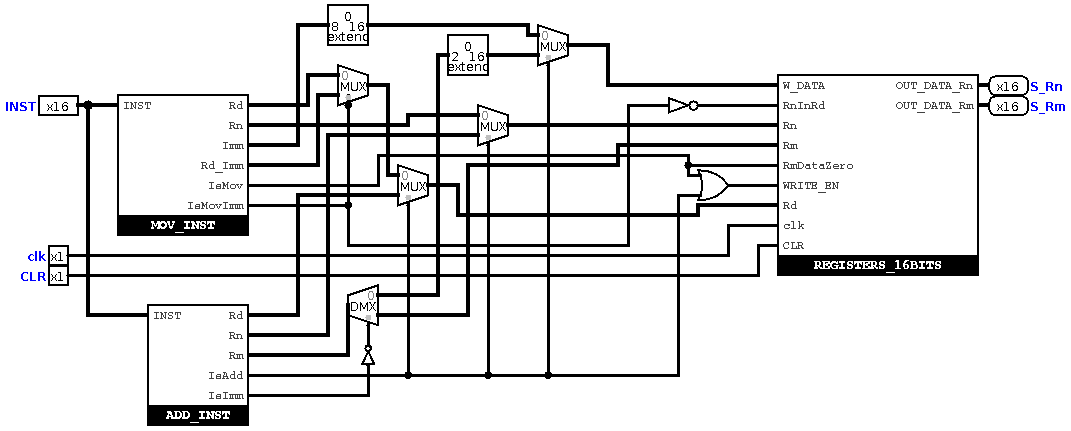
\includegraphics[width=1\textwidth]{src/Et4_DECODE.png}
    \caption{Bloc Decode}
    \label{decode_img}
\end{figure}

\paragraph{Définition des entrées:}
\begin{itemize}
    \item     INST: instruction à effectuer
    \item     clk: horloge
    \item     CLR: reset
\end{itemize}

\paragraph{Définition des sorties:}
\begin{itemize}
    \item     S\_Rn: Registre source 2
    \item     S\_Rm: Registre source 1
\end{itemize}
\medskip
Les sorties des blocs \textbf{MOV\_INST} et \textbf{ADD\_INST} étant toutes reliées à des entrées du bloc \textbf{REGISTERS\_16BITS}, le \textbf{DECODE} sera expliqué en décrivant les liens par rapport aux différentes entrées du bloc \textbf{REGISTER\_16BITS}. \medskip \\
\textbf{W\_DATA}: cette entrée est reliée aux sorties \textbf{Imm} du \textbf{MOV\_INST} et \textbf{Rm} du bloc \textbf{ADD\_INST}. Elle va prendre les valeurs immédiate en sortie de MOV et ADD, selon l'instruction donnée. Imm correpond à la valeur immédiate de l'instruction MOV et est sur 8 bit, elle passe donc dans un EXTEND qui permet de l'étendre à 16 bits. Rm est le registre source 1 de l'ADD. Il peut être sous forme de valeur immédiate ou non, c'est pourquoi il passe tout d'abord dans un démultiplexer, donc la sortie 0 correspond à une valeur immédiate, et va être reliée à un EXTEND qui va étendre la valeur sur 16 bit. Les deux valeurs immédiates (de MOV et de ADD) sur 16 bits sont reliées à un multiplexer. Ce dernier va envoyer la valeur en sortie de MOV si IsAdd (qui indique s'il y a une instruction ADD) est à 0, et la valeur en sortie de ADD si IsAdd est à 1.\\

\paragraph{RnInRd}: prend en entrée un NOT IsMovImm, qui indique que la valeur de l'instruction MOV n'est pas immédiate.\\

\paragraph{Rn}: prend en entrée le registre source 1, soit en sortie de \textbf{ADD\_INST} soit en sortie de \textbf{MOV\_INST}. Le bloc à choisir est déterminé par un multiplexer, qui est à 1 si IsAdd est activé.\\

\paragraph{Rm}: prend en entrée le registre source en sortie de \textbf{ADD\_INST}, si celui-ci n'est pas une valeur immédiate (vérifié par un multiplexer).\\

\paragraph{RmDataZero}:\footnote{Cette instruction aurait pu être gérée comme un ADD mais nous avons préféré garder cela comme un MOV} est activé si on a une instruction MOV, puisqu'elle ne possède qu'un registre source, il faut mettre la valeur contenue dans Rm à 0. Ainsi, elle est reliée la sortie IsMov, qui indique s'il s'agit a bien une instruction MOV.\\

\paragraph{WRITE\_EN}: s'active si on a une instruction MOV ou ADD. Ainsi, est relié à une porte OR qui prend en entrée IsAdd et IsMov.\\

\paragraph{Rd}: l'entrée Rd du REGISTER prend en entrée la sortie Rd du bloc \textbf{ADD\_INST} ou du bloc \textbf{MOV\_INST}, selon l'instruction voulue (choisie par un multiplexer dont la valeur est déterminée par IsAdd). Le registre destination du bloc \textbf{MOV\_INST} peut être une valeur immédiate ou non, raison pour laquelle il y a un multiplexer prenant en entrée les valeurs immédiate (qu'il prend en compte à 1) et non immédiate de ce bloc (qu'il prend en compte à 0), et qui passe à 1 lorsque IsMovImm (qui indique si la valeur est immédiate) est activée.
\medskip \\
Les deux dernière entrées du bloc (clk et CLR) sont simplement l'horloge et le reset.

\subsection{main}
\begin{figure}[H]
    \centering
    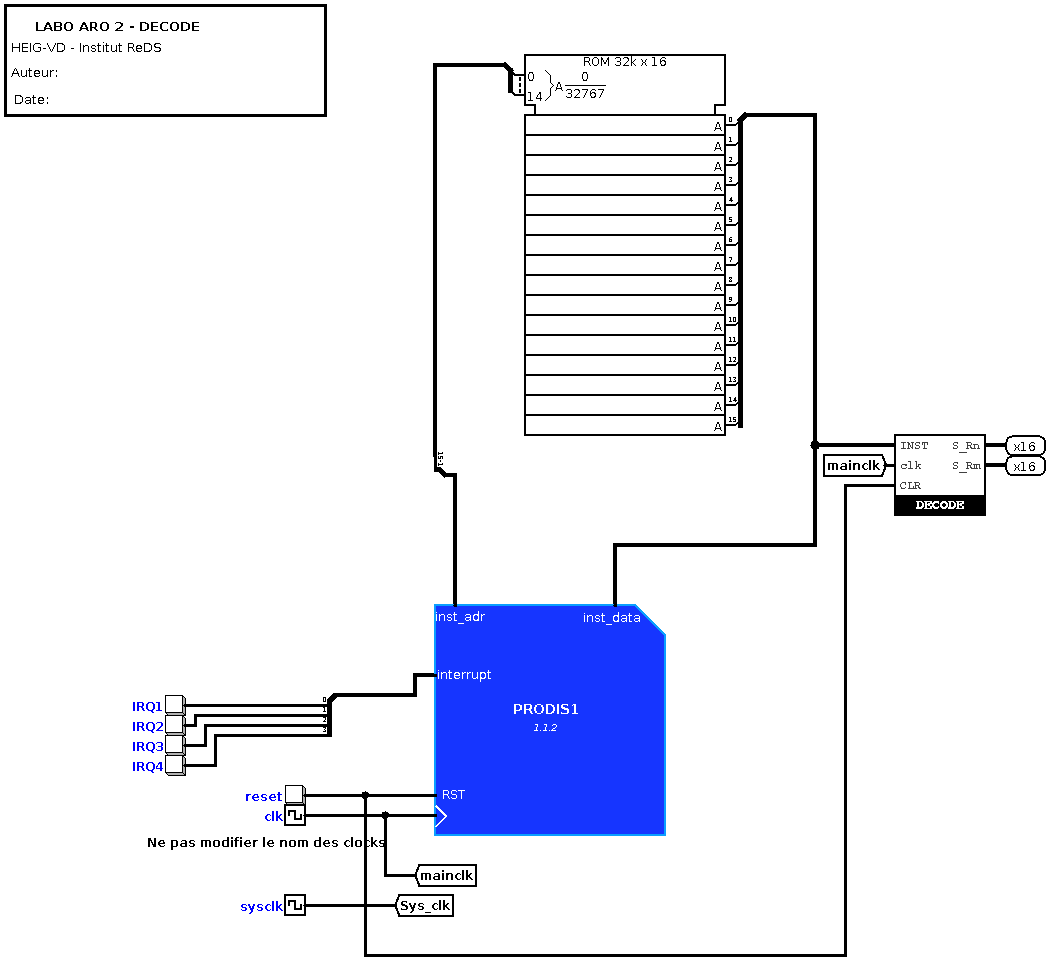
\includegraphics[width=1\textwidth]{src/Et4_main.png}
    \caption{Main program}
    \label{main_img}
\end{figure}

Le circuit main nous a permis de contrôler le bon fonctionnement de notre DECODE. Nous avions en instruction: \\


\begin{tabular}{|c|c|c|c|}
    
    \hline
    INST & Rd & Rn  & Rm  \\
    \hline
    MOV  & r1 & \#2  &    \\
    \hline
    MOV  & r3 & \#25 &    \\
    \hline
    ADD  & r2 & r1   & r3 \\
    \hline
    MOV  & r1 & \#12 &    \\
    \hline
    ADD  & r0 & r1   & r2 \\
    \hline
    MOV  & r3 & r0   &    \\
    \hline
\end{tabular}

\pagebreak
Le chronogramme suivant a permis de contrôler la bonne éxécution des instructions présentes dans le fichier fourni main.S décrit ci-dessus.
Toutes les valeurs sont en hexadécimal.
\begin{itemize}
    \item     INST: instruction courante
    \item     R0 à R3: registre et leur valeur
    \item    W\_DATA: valeur immédiate courante si utilisé
    \item    OUT\_DATA\_Rm: sortie actuelle du registre Rm
    \item    OUT\_DATA\_Rn: sortie actuelle du registre Rn    
    \item    Rd: Registre destination utilisé
    \item    Rn: Registre source 2 utilisé
    \item    Rm: Registre source 1 utilisé
\end{itemize}
On voit bien que les registres stockent les valeurs qui sont écrite dans le fichier et qu'ils sont correctement sélectionnés grâce aux entrées Rd, Rn et Rm.\\
La sortie OUT\_DATA\_Rm et l'entrée Rm est à 0 lors de l'instruction 0x210C et 0x1C03, car c'est une instruction MOV donc elle doit être nulle sinon elle altére le résultat de W\_DATA.\\

\begin{figure}[H]
    \centering
    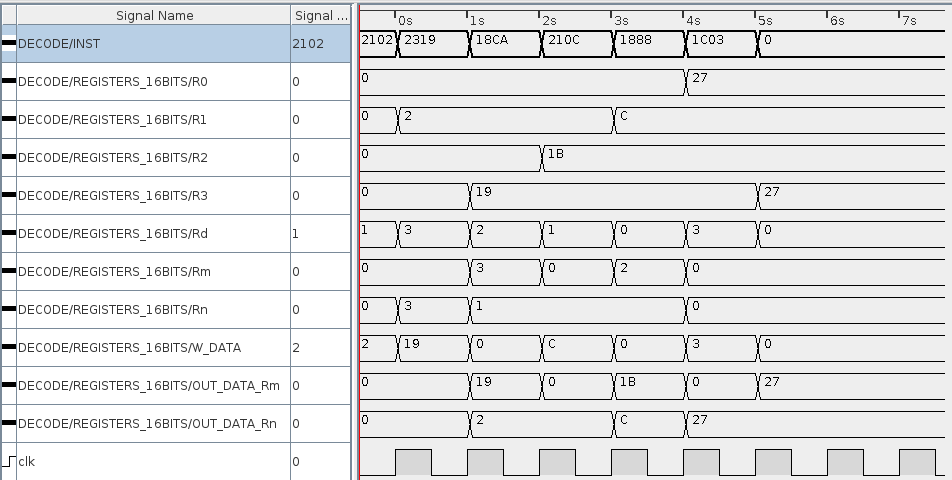
\includegraphics[width=1.3\textwidth]{src/Et4_CHRONO_MAIN.png}
    \caption{Chonogramme decode}
    \label{chrono_decode}
\end{figure}
\pagebreak

Pour s'assurer de la validité des données présentes dans les registres de la banque de regitres, voici le détail du résultat des instructions dans chaque registre:
\begin{enumerate}
    \item r1 $\leftarrow$ 0x0002
    \item r3 $\leftarrow$ 0x0019
    \item r2 $\leftarrow$ 0x001b
    \item r1 $\leftarrow$ 0x000c
    \item r0 $\leftarrow$ 0x0027
    \item r3 $\leftarrow$ 0x0027
\end{enumerate}

À la fin des instructions, il y a donc: r0=0x0027, r1=0x000c, r2=0001b et r3=0x0027.
Dans le chronogramme, il y a effectivement les valeurs suivantes à chaque registre. \\
En sortie du main, dans Rn et Rm se trouvent les valeurs 0x0027, et il s'agit bien des valeurs qu'on avait en registre source et qui ont été mises dans le registre destination.

\section{Conclusion}
Ce laboratoire était la suite directe du laboratoire fetch, et a permis de faire les liens entre ces deux parties. Comme pour le laboratoire précédent, plusieurs petits circuits ont été 
créés séparéments pour ensuite les réunir dans le decode, pour plus de lisibilité.\\
Le bloc permettant de reconnaître l'instruction MOV avait déjà été réalisé pour la partie fetch et nous avons pu nous en inspirer. L'ensemble de ce laboratoire nous permis de mieux comprendre le fonctionnement de la partie decode, et des instructions MOV et ADD.\\
L'instruction 1c03 nous a posé problème car nous avions mal géré la détection du MOV et c'est grâce à cela que nous avons compris que le MOV n'était qu'une instruction ADD avec une valeur immédiate à 0.

\section{Annexe}
\subsection{Test de la banque de registre}
Dans la 1ère capture d'écran, le Registre 3 à comme valeur 0x201b et il est sélectionné en tant que Rd, la donnée choisie est affichée correctement dans OUT\_DATA.\\
Ensuite l'entrée RnInRd est activée donc ce n'est pas une valeur immédiate qui sera écrite dans le Regsitre 1 (sélectionné par Rn) mais bien la donnée contenue dans R3.\\

\begin{figure}[H]
    \centering
    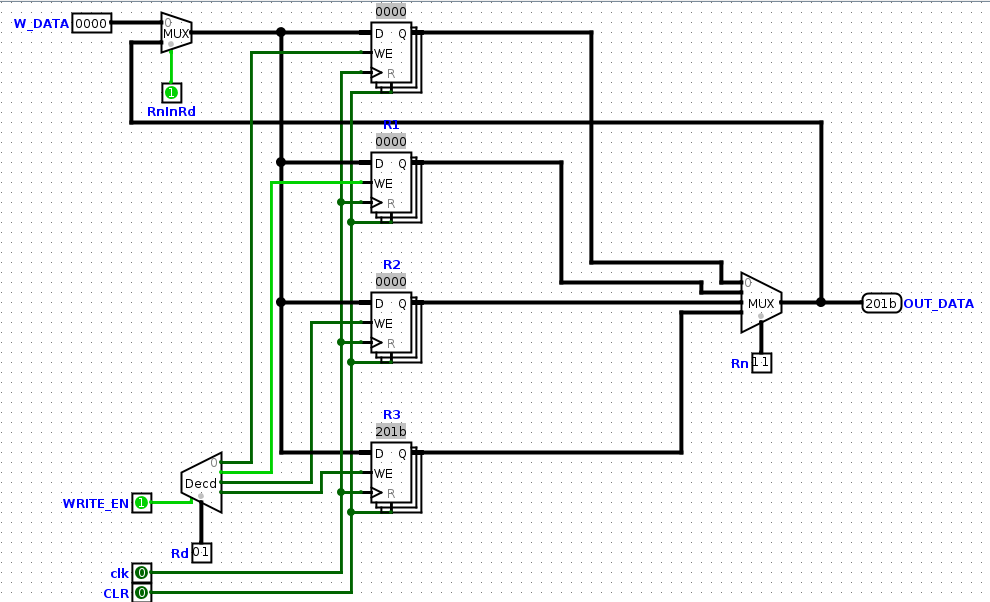
\includegraphics[width=1.3\textwidth]{src/TEST_REGISTERS_1.png}
    \caption{Test avant activation de clk}
    \label{test_1}
\end{figure}
    
Après activation de l'horloge, la valeur de R3 à bien été écrite dans le registre 1.    
\begin{figure}[H]
    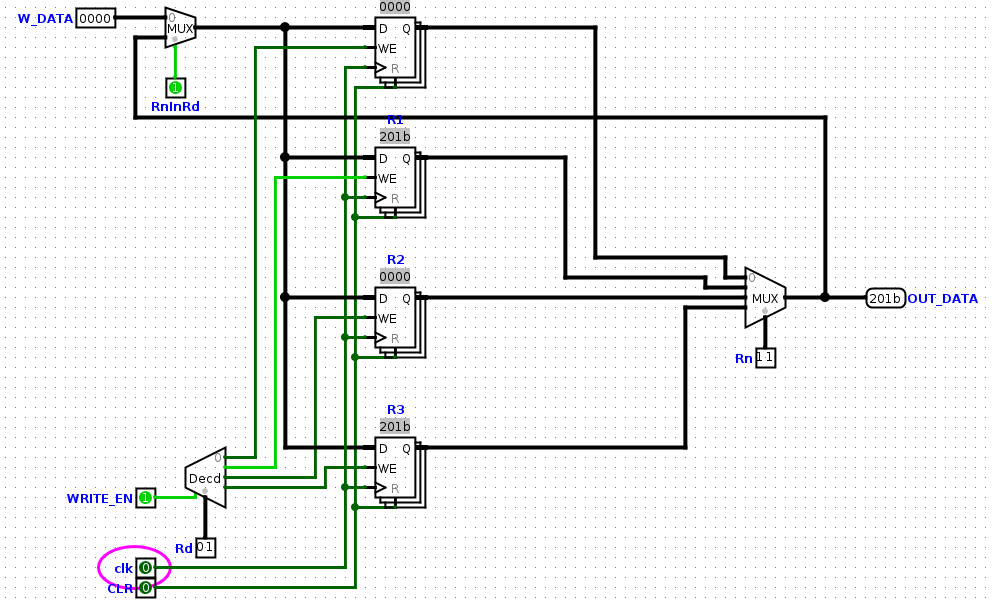
\includegraphics[width=1.3\textwidth]{src/TEST_REGISTERS_2.png}
    \caption{Test après activation de clk}
    \label{test_2}
\end{figure}



\end{document}